\documentclass{article}
\usepackage[letterpaper]{geometry}
\usepackage{graphicx}
\graphicspath{ {./images/} }

\title{Pavon The Game - A technical overview}
\date{Enero - 2025}
\author{by Oscar G. Pav\'on}



\begin{document}
  \pagenumbering{gobble}
  \maketitle
  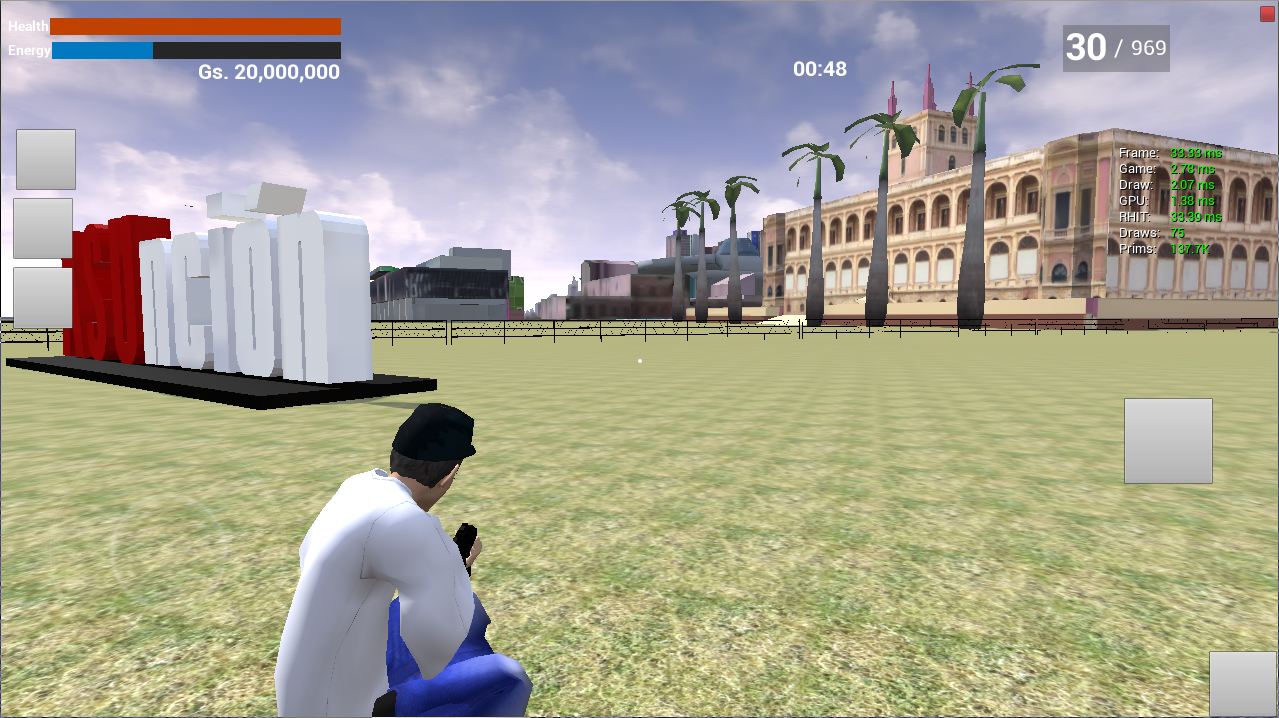
\includegraphics[width=\textwidth]{1.png}

  \pagenumbering{arabic}

  \newpage
  \section{Introduction}
  In the proccess for aquire knowleghe at some point of our life we need to share the knowleghe.
  This is a technical book intended to describe the proccess of making a game. My own game, for aquire technicals habilities

  \newpage
  \section{The 3D art}
  
  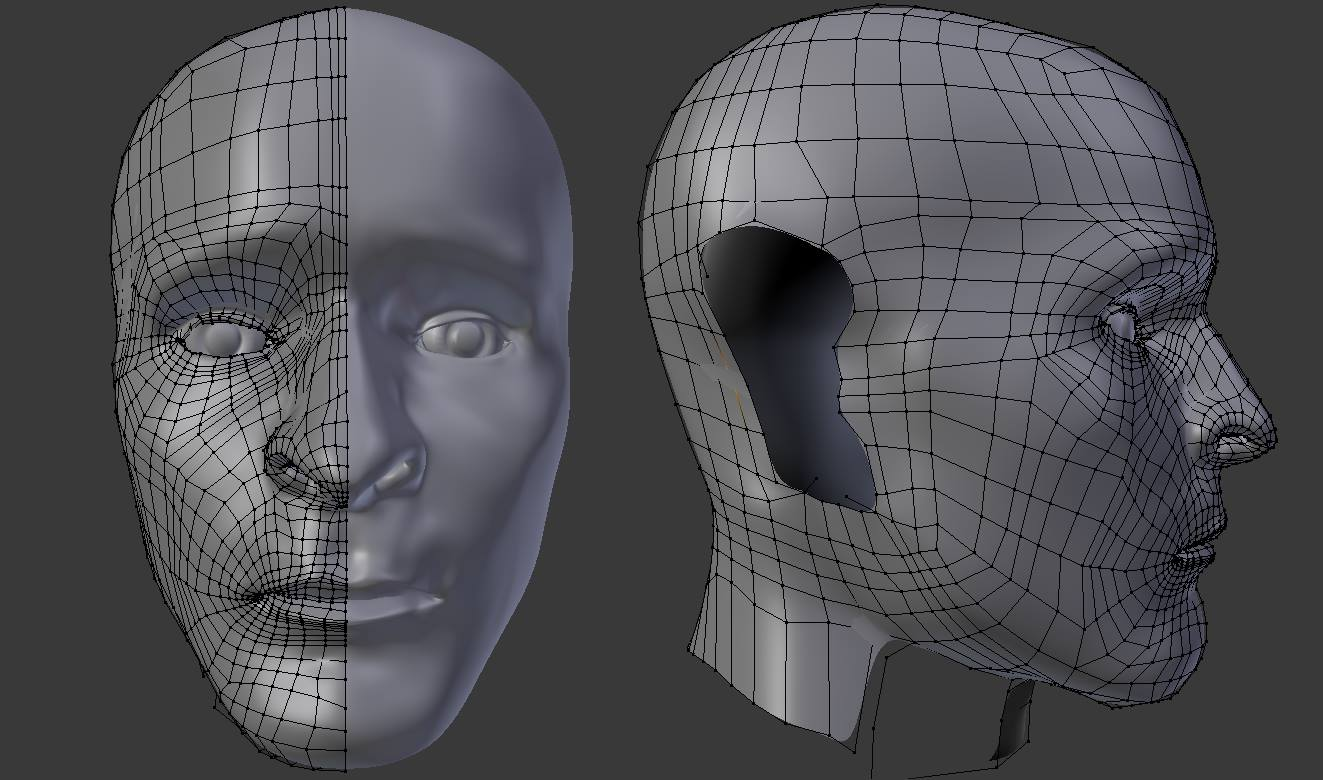
\includegraphics[width=\textwidth]{4.jpg}
  The head was allway a challange


  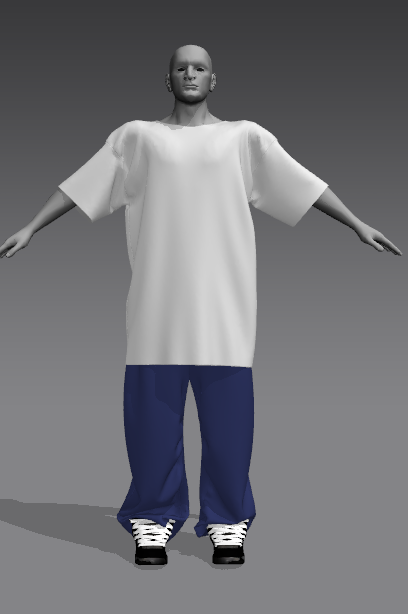
\includegraphics[width=\textwidth]{3.png}
  I used Marvelous Designer for create the cloth

  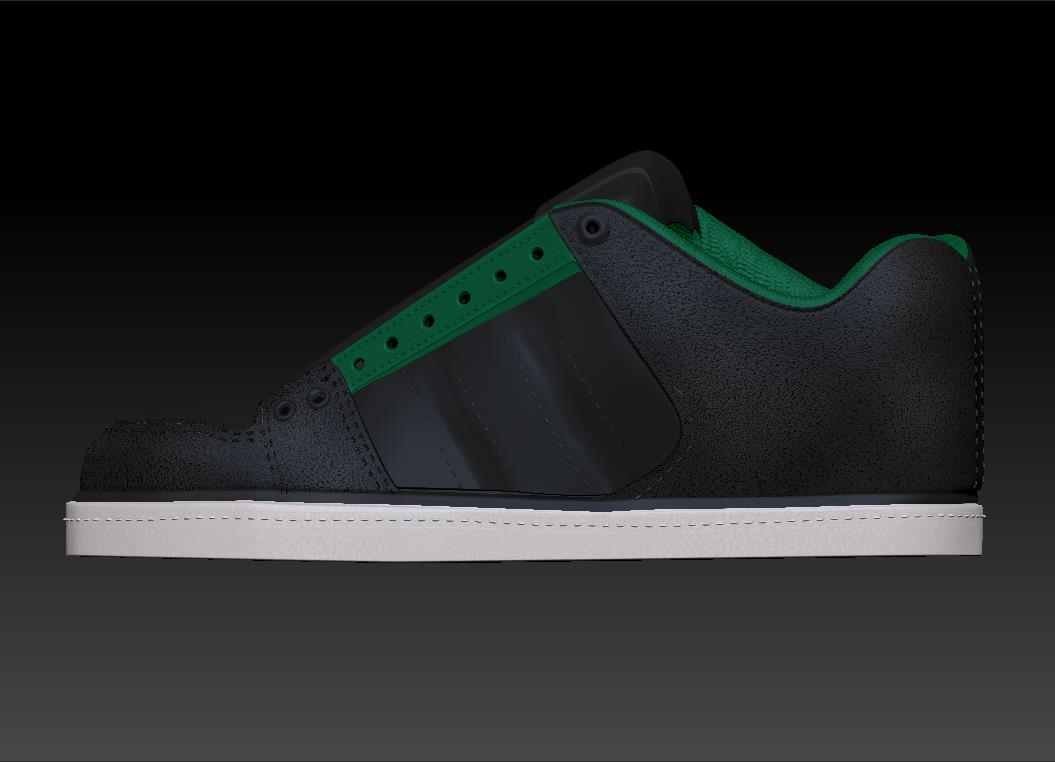
\includegraphics[width=\textwidth]{5.jpg}
  This is in ZBrush for adding details to the shoe

  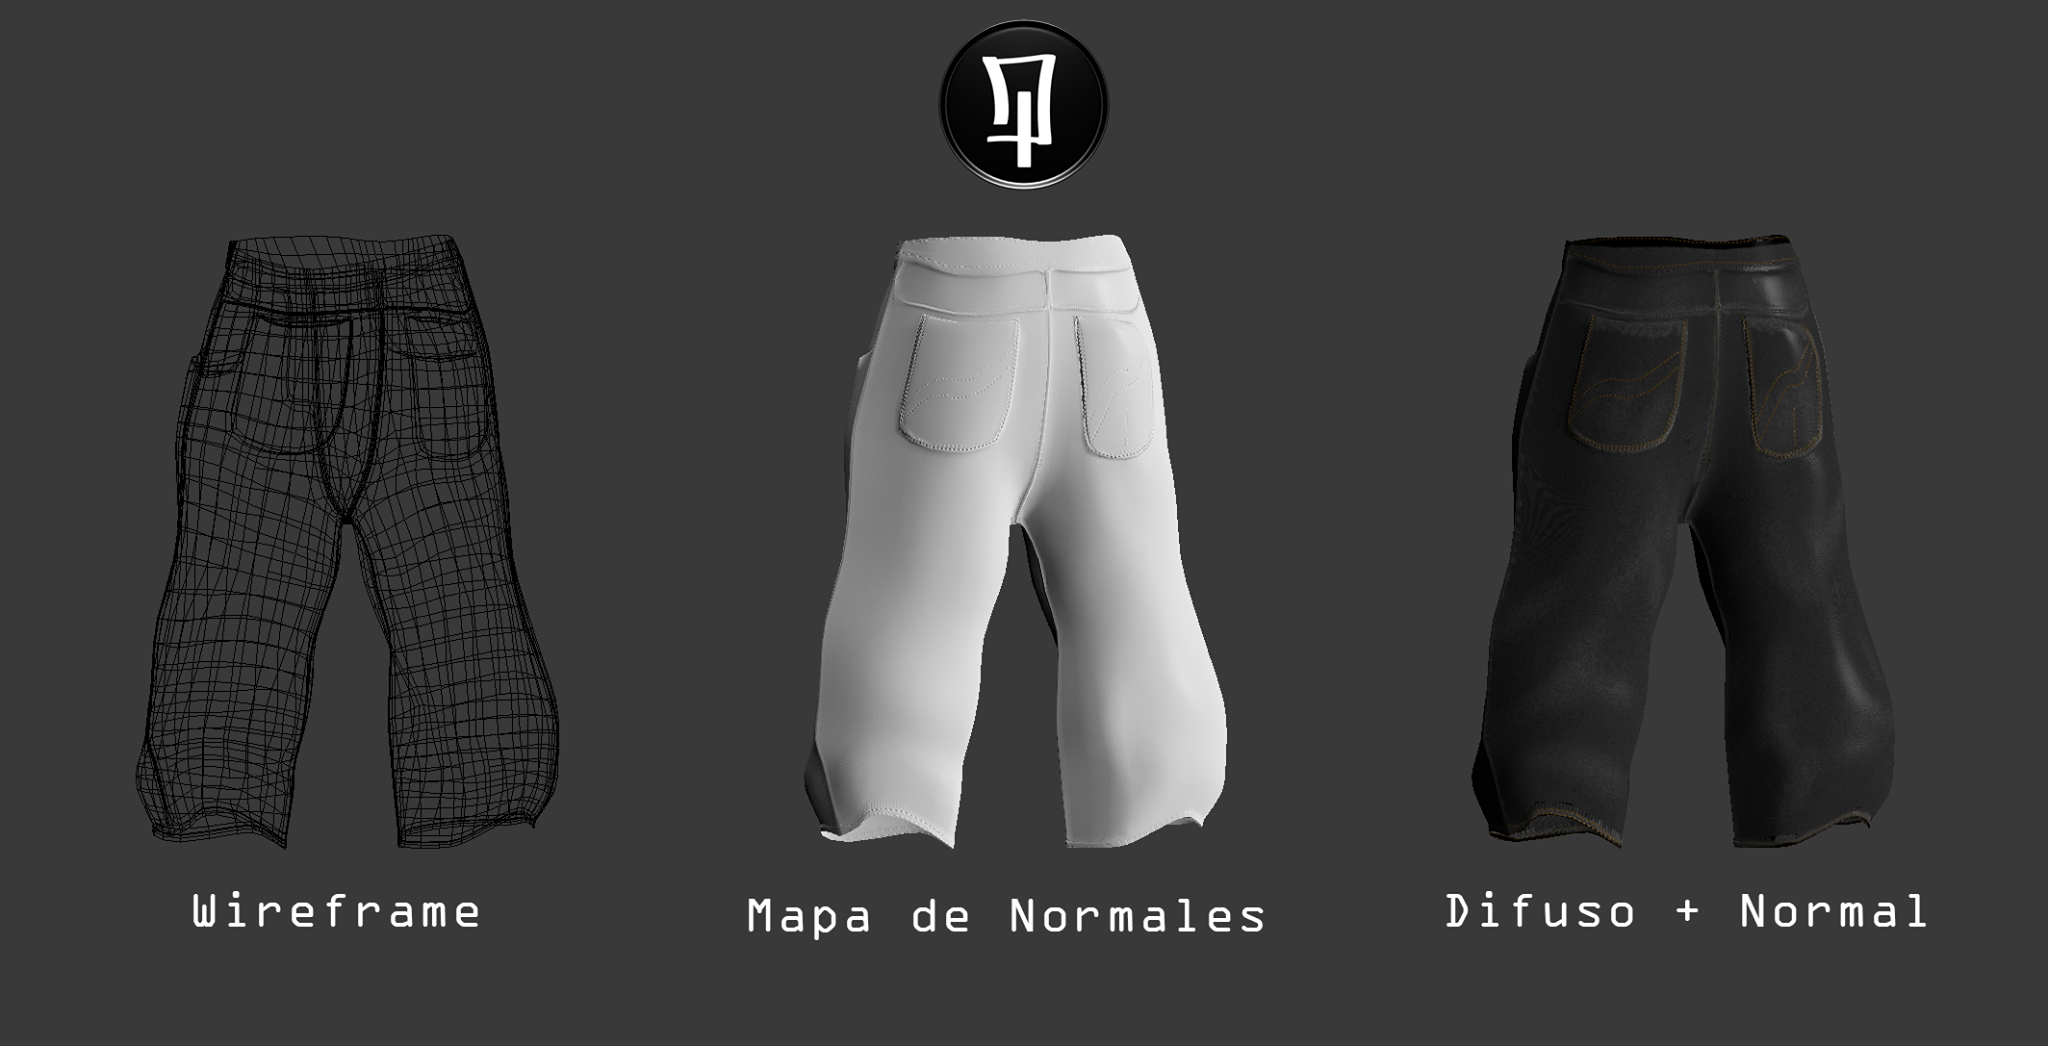
\includegraphics[width=\textwidth]{6.png}

  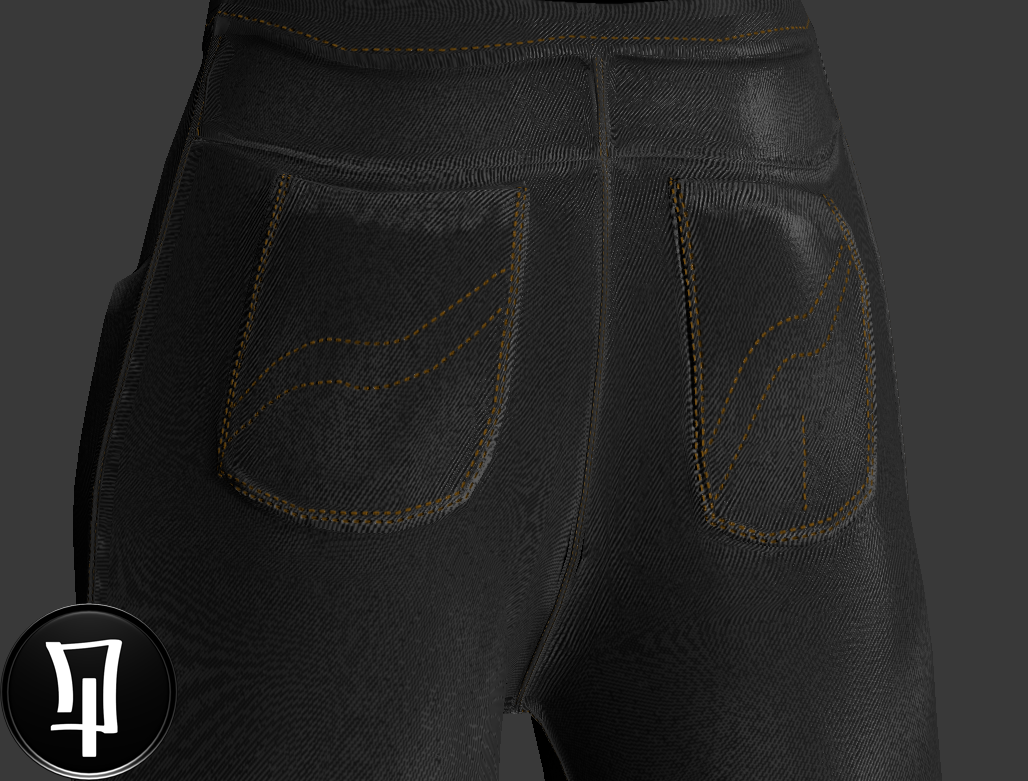
\includegraphics[width=\textwidth]{7.png}
  
  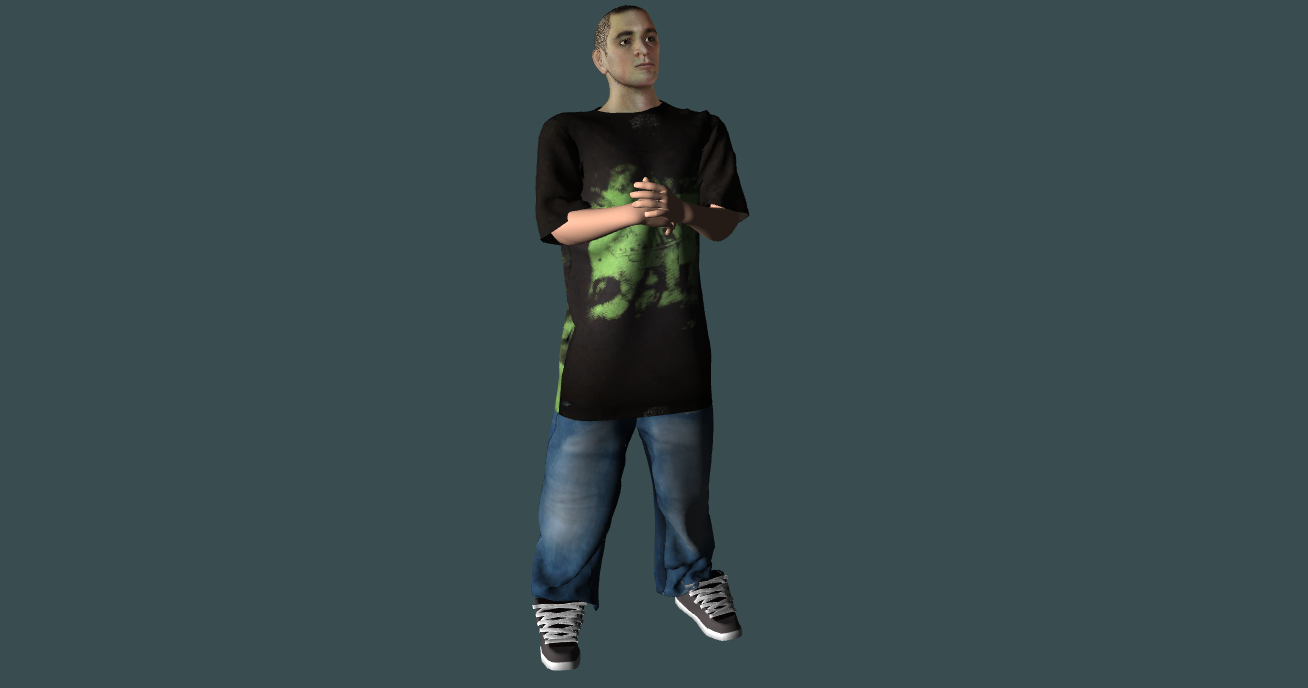
\includegraphics[width=\textwidth]{16.png}
  
  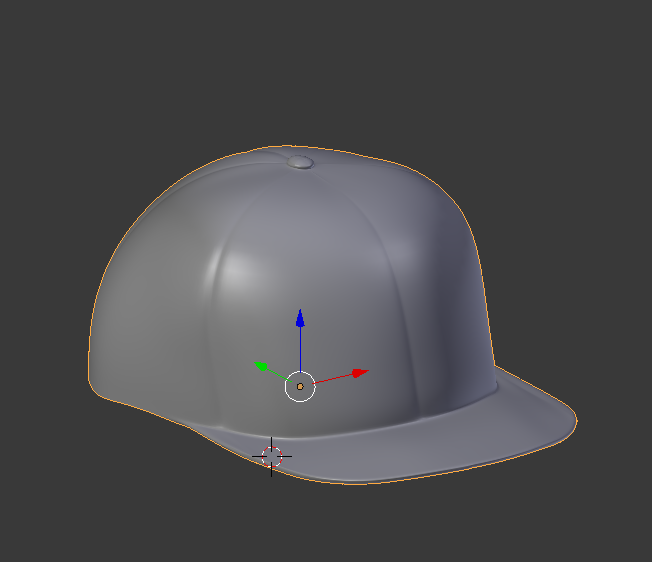
\includegraphics[width=\textwidth]{8.png}

  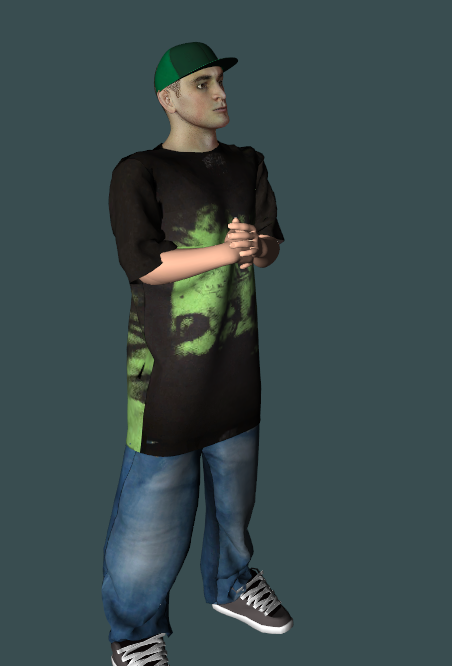
\includegraphics[width=\textwidth]{9.png}
  We have the main character now


  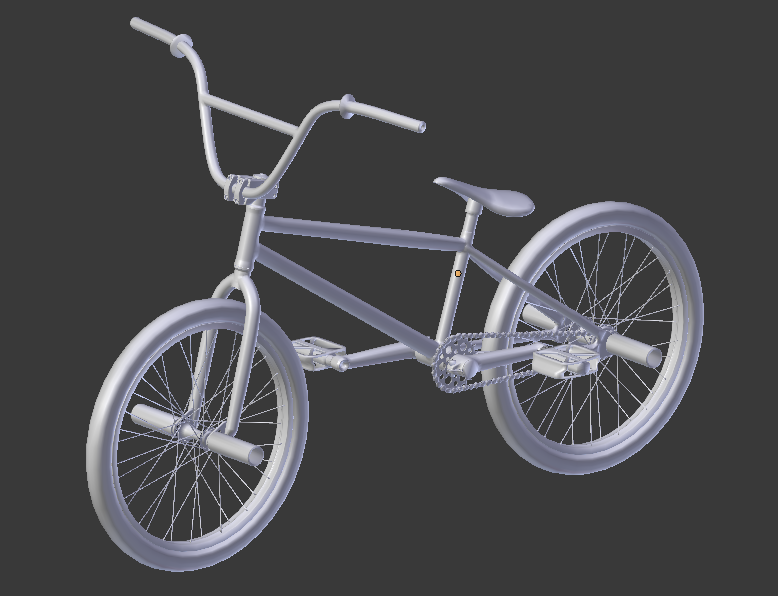
\includegraphics[width=\textwidth]{12.png}

  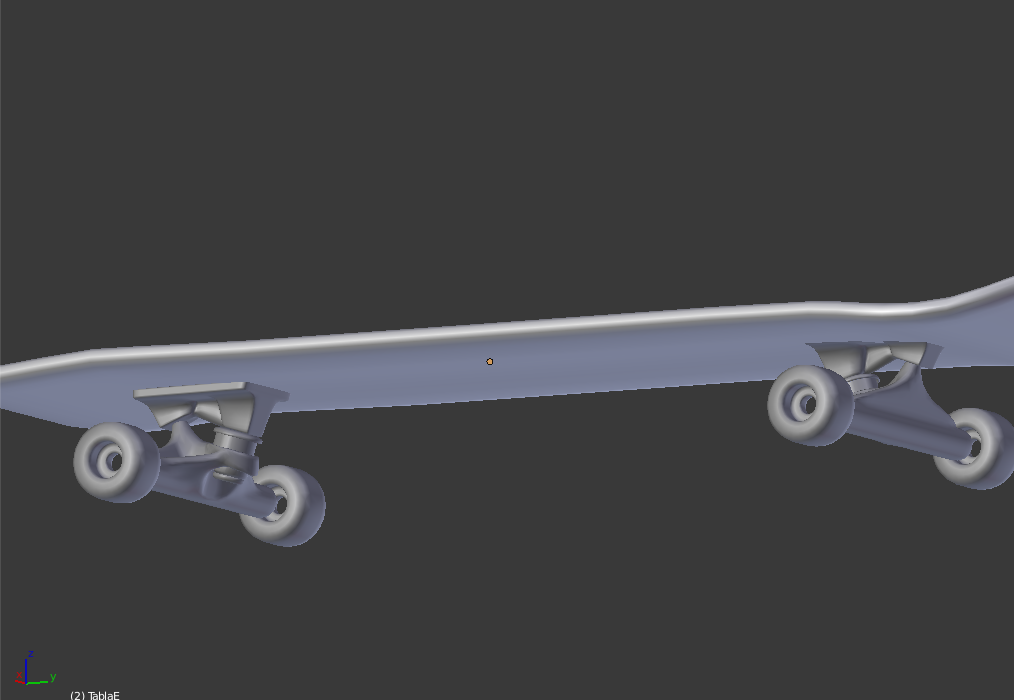
\includegraphics[width=\textwidth]{13.png}
  
  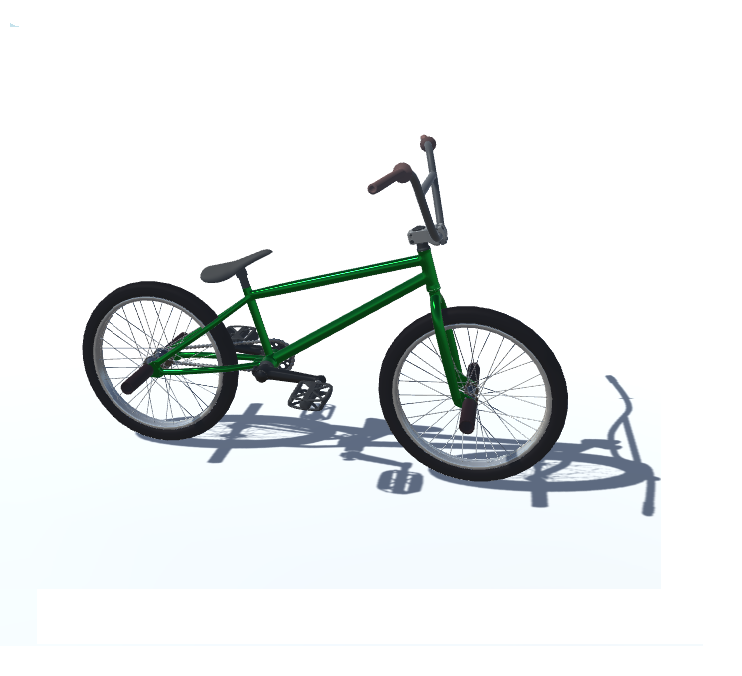
\includegraphics[width=\textwidth]{15.png}

  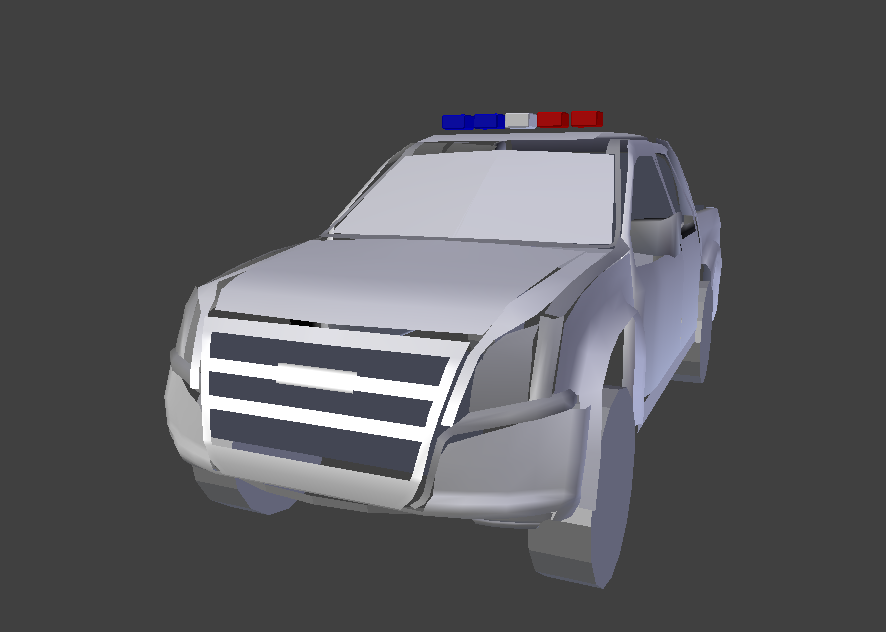
\includegraphics[width=\textwidth]{2.png}
  
  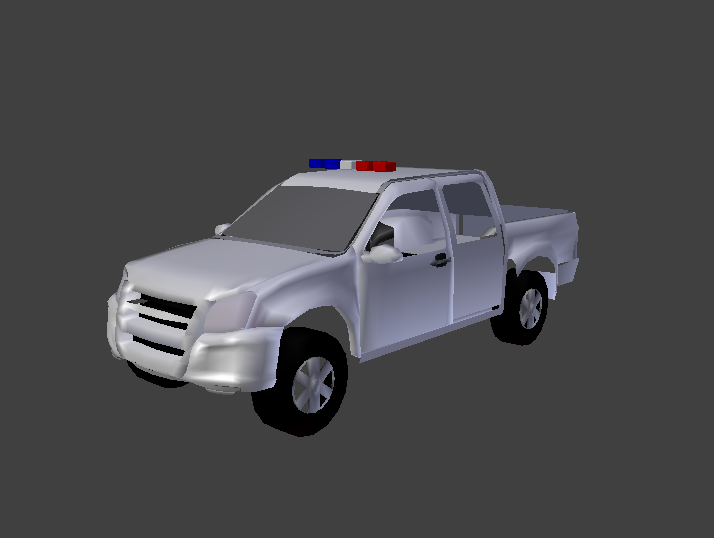
\includegraphics[width=\textwidth]{11.png}

  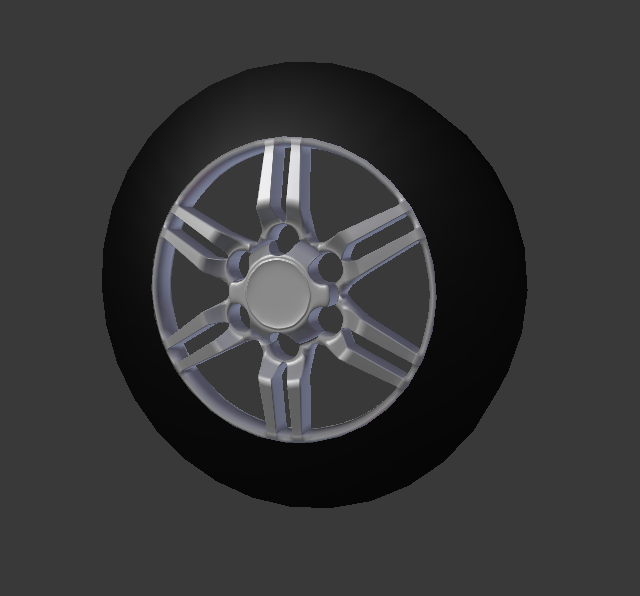
\includegraphics[width=\textwidth]{14.png}
\end{document}
